% The format (A5) is selected to facilitate reading on small
% devices and should NOT be changed. 
\documentclass[a5paper,10pt,oneside]{article}

% The package babel is loaded for Swdish with Swedish hyphenation,
% replaces "Contents" with "Innehållsförteckning, "References"
% with "Litteraturförteckning", etc.
\usepackage[swedish]{babel}

\usepackage[T1]{fontenc}

% The package "inputenc" lets us specify what character encoding
% has been used to save the .tex file. If your computer runs
% Linux, the encoding is probably "utf8" by default, while under
% Windows the default will probably be "latin1" The wrong
% character encoding may give strange signs instead of "å", "ä"
% and "ö" or may result in compilation errors.

%\usepackage[latin1]{inputenc} % Probably right if you use Windows
\usepackage[utf8]{inputenc}  % Probably right if you use Linux

% The packages listed below are optional and can be removed if you
% don't use them 
\usepackage{graphicx} 
\usepackage{cite}
\usepackage{url}
\usepackage{ifthen}
\usepackage{listings}	

% These two lines set up options for the listings package and
% can be removed if you don't use it, or changed if you, e.g, 
% use another language than Java. 
% For more information about the listings package see:
% ftp://ftp.tex.ac.uk/tex-archive/macros/latex/contrib/listings/listings.pdf
\def \lstlistingname {Kodexempel}
\lstset{language=Java,tabsize=3,numbers=left,frame=L,floatplacement=hbtp}


\usepackage{ifpdf}
\ifpdf
	\usepackage[hidelinks]{hyperref}
\else
	\usepackage{url}
\fi


% Change NR and TITLE below to appropriate values
\title{Tema NR: 3 Träd}

% Write the name and user namn for all participants in the group here.
% Separate persons with \and
\author{Oscar Törnquist \url{osta3589} \and Emil Rosell \url{emro9957}}



\begin{document}
\maketitle

\section*{Dubbelrotationer}

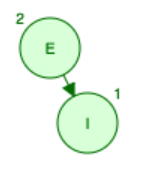
\includegraphics[scale=0.7]{em}
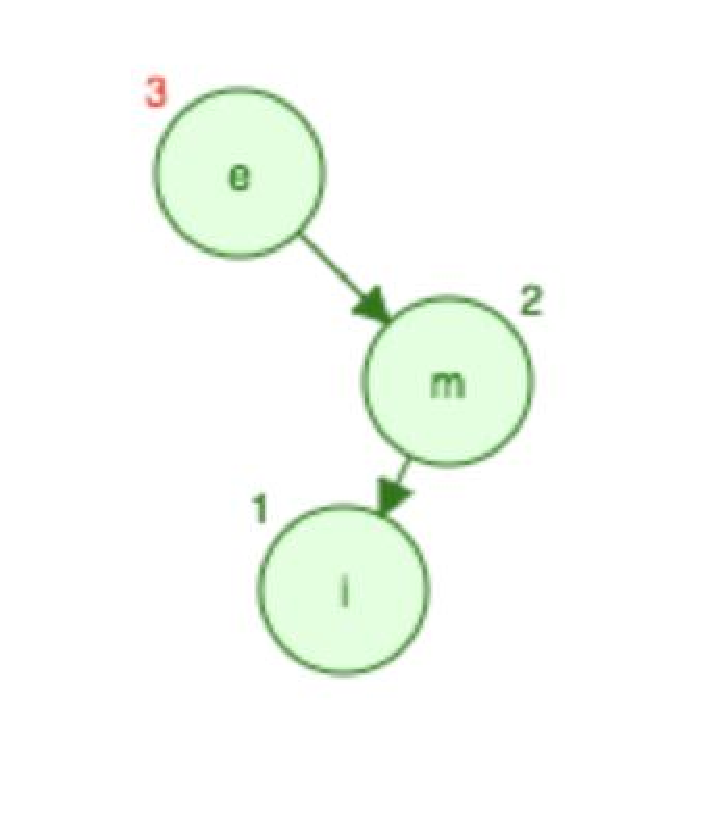
\includegraphics[scale=0.2]{emiBefore}
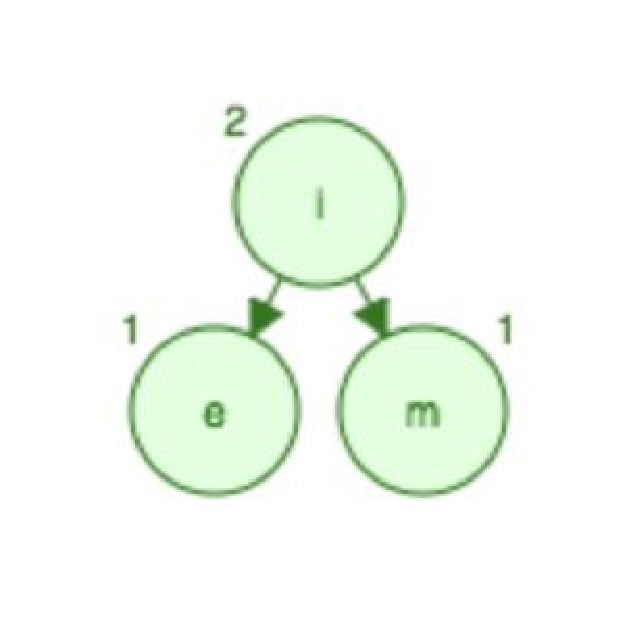
\includegraphics[scale=0.3]{emiAfter}

Vi börjar med att lägga till ett $e$ följt av ett $m$ utan problem. När vi sedan lägger till ett i stöter vi på ett problem och det sker en enkel rotation. När $i$ läggs till hamnar den förs till vänster i m noden vilket gör att det blir obalans. För att bli av med obalansen flyttas i upp ett steg och blir rotnoden. Eftersom e kommer före i så läggs e till vänster bland barnnoderna och m som kommer efter i läggs till höger. 

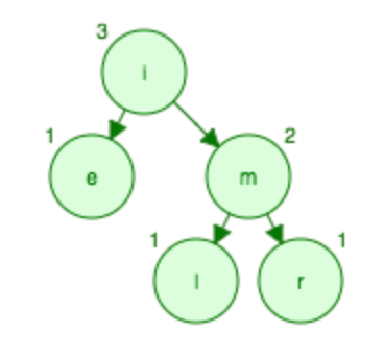
\includegraphics[scale=0.45]{emilr}
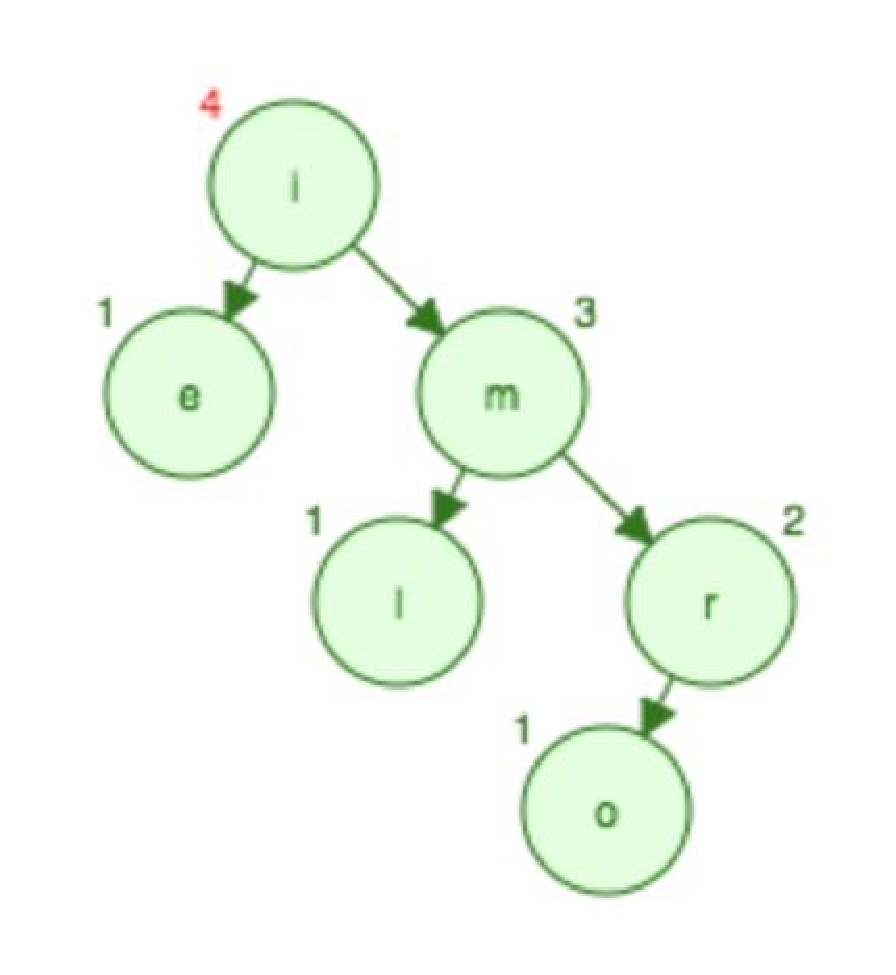
\includegraphics[scale=0.25]{emilroBefore}
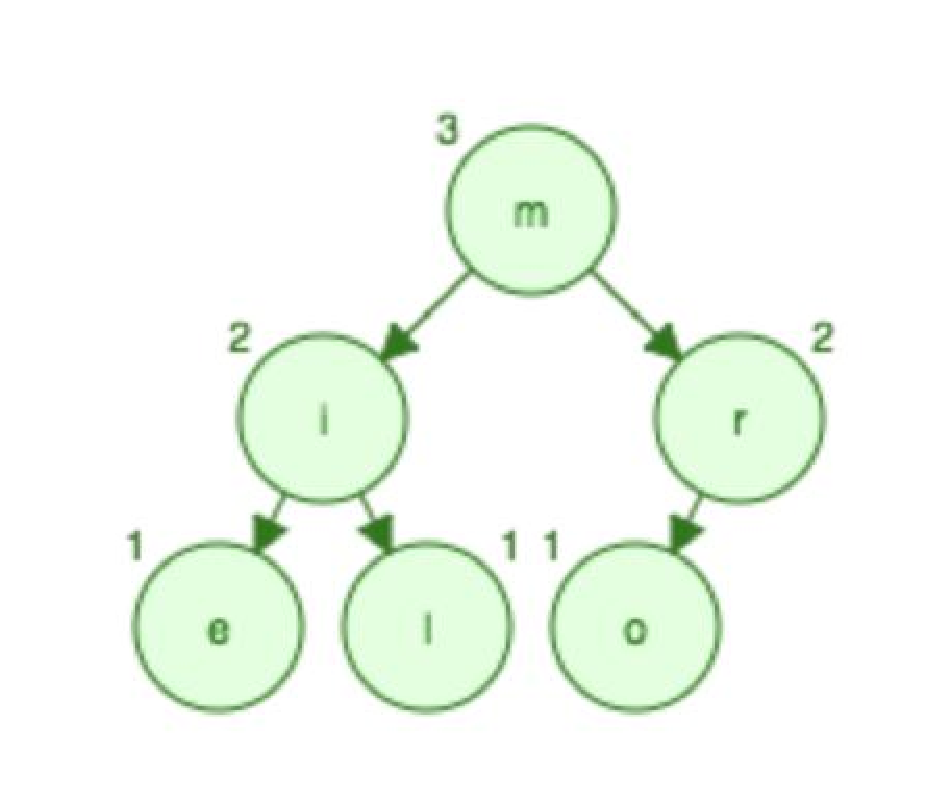
\includegraphics[scale=0.25]{emilroAfter}

Vi kan sedan lägga till l och r utan problem, men när vi lägger till o får vi obalans.
\end{document}
